

\chapter{Single and double scenario, KFold Validation}

Starting with fitting randomly the classifiers, there are some statistics of the data used for the first test: \\
 {\def\arraystretch{1.3} 
 \begin{table}[H] 
\centering 
\begin{tabular}{|l|l|l|} 
\hline 
  &count train  &count test  \\ \hline
mess  &97  &253  \\ \hline
tele  &335  &715  \\ \hline
what  &219  &481  \\ \hline
mess\_mess  &99  &251  \\ \hline
tele\_mess  &113  &237  \\ \hline
what\_mess  &93  &257  \\ \hline
mess\_tele  &89  &261  \\ \hline
what\_tele  &103  &247  \\ \hline
mess\_what  &106  &244  \\ \hline
original  &111  &239  \\ \hline
\end{tabular} 
\end{table} }
\section{Logistic regression results:} 
Confusion matrix with number of sample and with normalization:
 {\def\arraystretch{1.3} 
 \begin{table}[H] 
\centering 
\begin{tabular}{|l|l|l|l|l|l|l|l|l|l|l|} 
\hline 
  &m  &t  &w  &m\_m  &m\_t  &m\_w  &t\_m  &t\_w  &w\_m  &original  \\ \hline
mess  &181  &0  &0  &45  &4  &23  &0  &0  &0  &0  \\ \hline
tele  &0  &700  &0  &0  &0  &0  &9  &6  &0  &0  \\ \hline
what  &0  &0  &414  &0  &0  &0  &0  &0  &63  &4  \\ \hline
mess\_mess  &22  &0  &0  &217  &6  &6  &0  &0  &0  &0  \\ \hline
tele\_mess  &0  &0  &0  &0  &225  &12  &0  &0  &0  &0  \\ \hline
what\_mess  &0  &0  &0  &0  &77  &180  &0  &0  &0  &0  \\ \hline
mess\_tele  &0  &248  &0  &0  &0  &0  &6  &7  &0  &0  \\ \hline
what\_tele  &0  &7  &0  &0  &0  &0  &0  &240  &0  &0  \\ \hline
mess\_what  &0  &1  &180  &0  &0  &0  &0  &0  &63  &0  \\ \hline
original  &0  &0  &0  &0  &0  &0  &0  &0  &0  &239  \\ \hline
\end{tabular} 
\end{table} }

 \begin{figure}[H] 
\centering 
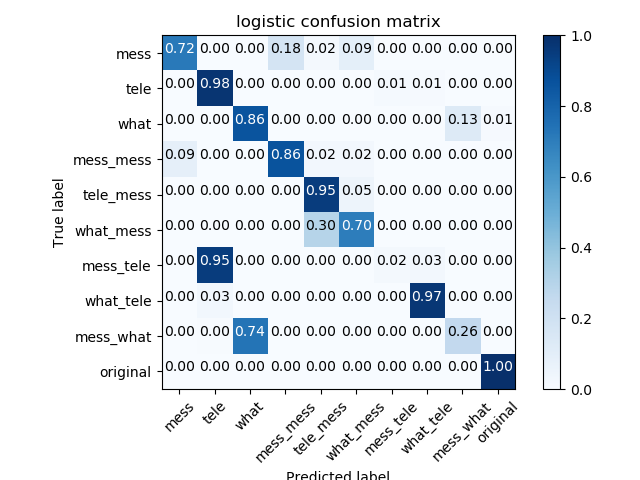
\includegraphics[scale=.6]{images/lr_initial_single_double_complete.png} 
\caption{logistic regression, last app classified} 
\end{figure} 


Result of the KFold validation with 10 bins:
 {\def\arraystretch{1.3} 
 \begin{table}[H] 
\centering 
\begin{tabular}{|l |l |l |l |l |l |l |l |l |l |}  
\hline 
0.8248&
0.8029&
0.7737&
0.8029&
0.7299&
0.8162&
0.7426&
0.8088&
0.7868&
0.8015\\ \hline  

\end{tabular} 
\end{table} }

The mean is : 0.789019\section{Linear Support Vector Machine results:} 
Confusion matrix with number of sample and with normalization:
 {\def\arraystretch{1.3} 
 \begin{table}[H] 
\centering 
\begin{tabular}{|l|l|l|l|l|l|l|l|l|l|l|} 
\hline 
  &m  &t  &w  &m\_m  &m\_t  &m\_w  &t\_m  &t\_w  &w\_m  &original  \\ \hline
mess  &195  &0  &0  &37  &4  &17  &0  &0  &0  &0  \\ \hline
tele  &0  &681  &0  &0  &0  &0  &34  &0  &0  &0  \\ \hline
what  &0  &0  &386  &0  &0  &0  &0  &0  &91  &4  \\ \hline
mess\_mess  &26  &0  &0  &217  &5  &3  &0  &0  &0  &0  \\ \hline
tele\_mess  &0  &0  &0  &0  &217  &20  &0  &0  &0  &0  \\ \hline
what\_mess  &0  &0  &1  &1  &44  &211  &0  &0  &0  &0  \\ \hline
mess\_tele  &0  &232  &0  &0  &0  &0  &29  &0  &0  &0  \\ \hline
what\_tele  &0  &5  &0  &0  &0  &0  &0  &242  &0  &0  \\ \hline
mess\_what  &0  &0  &145  &0  &1  &0  &0  &0  &98  &0  \\ \hline
original  &0  &0  &0  &0  &0  &0  &0  &0  &0  &239  \\ \hline
\end{tabular} 
\end{table} }

 \begin{figure}[H] 
\centering 
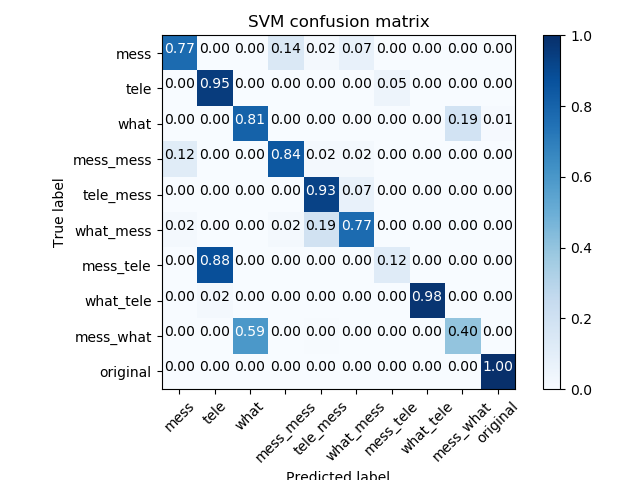
\includegraphics[scale=.6]{images/lsvm_initial_single_double_complete.png} 
\caption{linear SVM, last app classified} 
\end{figure} 


Result of the KFold validation with 10 bins:
 {\def\arraystretch{1.3} 
 \begin{table}[H] 
\centering 
\begin{tabular}{|l |l |l |l |l |l |l |l |l |l |}  
\hline 
0.8394&
0.7956&
0.7810&
0.8321&
0.7226&
0.8162&
0.7574&
0.8015&
0.7794&
0.8088\\ \hline  

\end{tabular} 
\end{table} }

The mean is : 0.793404\section{Random forest results:} 
Confusion matrix with number of sample and with normalization:
 {\def\arraystretch{1.3} 
 \begin{table}[H] 
\centering 
\begin{tabular}{|l|l|l|l|l|l|l|l|l|l|l|} 
\hline 
  &m  &t  &w  &m\_m  &m\_t  &m\_w  &t\_m  &t\_w  &w\_m  &original  \\ \hline
mess  &196  &0  &0  &41  &1  &14  &0  &0  &1  &0  \\ \hline
tele  &0  &579  &0  &0  &0  &0  &133  &3  &0  &0  \\ \hline
what  &0  &0  &344  &0  &0  &0  &0  &0  &134  &3  \\ \hline
mess\_mess  &49  &0  &0  &197  &3  &1  &0  &0  &1  &0  \\ \hline
tele\_mess  &2  &0  &0  &0  &222  &13  &0  &0  &0  &0  \\ \hline
what\_mess  &14  &0  &7  &16  &18  &200  &0  &0  &2  &0  \\ \hline
mess\_tele  &0  &187  &0  &0  &0  &0  &71  &3  &0  &0  \\ \hline
what\_tele  &0  &3  &0  &0  &0  &0  &1  &243  &0  &0  \\ \hline
mess\_what  &1  &0  &173  &0  &0  &0  &0  &0  &70  &0  \\ \hline
original  &0  &0  &3  &1  &0  &1  &0  &0  &0  &234  \\ \hline
\end{tabular} 
\end{table} }

 \begin{figure}[H] 
\centering 
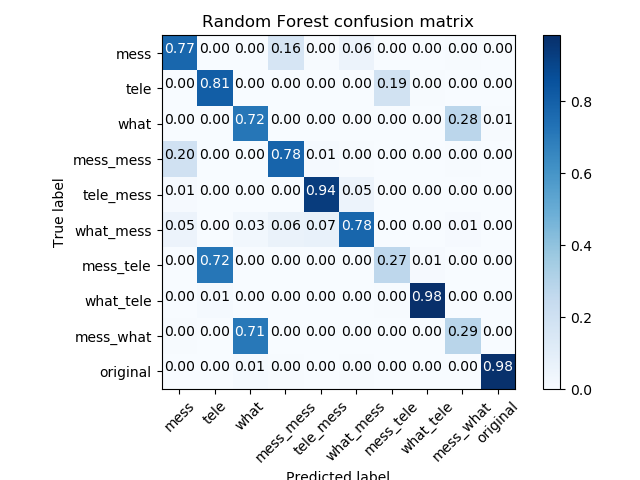
\includegraphics[scale=.6]{images/rf_initial_single_double_complete.png} 
\caption{random forest, last app classified} 
\end{figure} 


Result of the KFold validation with 10 bins:
 {\def\arraystretch{1.3} 
 \begin{table}[H] 
\centering 
\begin{tabular}{|l |l |l |l |l |l |l |l |l |l |}  
\hline 
0.7956&
0.8029&
0.7153&
0.8248&
0.6642&
0.8382&
0.7279&
0.7426&
0.6691&
0.7647\\ \hline  

\end{tabular} 
\end{table} }

The mean is : 0.754557